%% LyX 2.3.6.1 created this file.  For more info, see http://www.lyx.org/.
%% Do not edit unless you really know what you are doing.
\documentclass[12pt,preprint,3p]{elsarticle}
\usepackage[latin9]{inputenc}
\usepackage{float}
\usepackage{amsmath}
\usepackage{amssymb}
\usepackage{graphicx}

\makeatletter

%%%%%%%%%%%%%%%%%%%%%%%%%%%%%% LyX specific LaTeX commands.
%% Because html converters don't know tabularnewline
\providecommand{\tabularnewline}{\\}

%%%%%%%%%%%%%%%%%%%%%%%%%%%%%% User specified LaTeX commands.
%%
%% Copyright 2007, 2008, 2009 Elsevier Ltd
%%
%% This file is part of the 'Elsarticle Bundle'.
%% ---------------------------------------------
%%
%% It may be distributed under the conditions of the LaTeX Project Public
%% License, either version 1.2 of this license or (at your option) any
%% later version.  The latest version of this license is in
%%    http://www.latex-project.org/lppl.txt
%% and version 1.2 or later is part of all distributions of LaTeX
%% version 1999/12/01 or later.
%%
%% The list of all files belonging to the 'Elsarticle Bundle' is
%% given in the file `manifest.txt'.
%%

%% Template article for Elsevier's document class `elsarticle'
%% with numbered style bibliographic references
%% SP 2008/03/01
%%
%%
%%
%% $Id: elsarticle-template-num.tex 4 2009-10-24 08:22:58Z rishi $
%%
%%


%% Use the option review to obtain double line spacing
%% \documentclass[preprint,review,12pt]{elsarticle}

%% Use the options 1p,twocolumn; 3p; 3p,twocolumn; 5p; or 5p,twocolumn
%% for a journal layout:
%% \documentclass[final,1p,times]{elsarticle}
%% \documentclass[final,1p,times,twocolumn]{elsarticle}
%% \documentclass[final,3p,times]{elsarticle}
%% \documentclass[final,3p,times,twocolumn]{elsarticle}
%% \documentclass[final,5p,times]{elsarticle}
%% \documentclass[final,5p,times,twocolumn]{elsarticle}

%% if you use PostScript figures in your article
%% use the graphics package for simple commands
%% \usepackage{graphics}
%% or use the graphicx package for more complicated commands
%% \usepackage{graphicx}
%% or use the epsfig package if you prefer to use the old commands
%% \usepackage{epsfig}

%% The amssymb package provides various useful mathematical symbols
%% The amsthm package provides extended theorem environments
%% \usepackage{amsthm}

%% The lineno packages adds line numbers. Start line numbering with
%% \begin{linenumbers}, end it with \end{linenumbers}. Or switch it on
%% for the whole article with \linenumbers after \end{frontmatter}.
%% \usepackage{lineno}

%% natbib.sty is loaded by default. However, natbib options can be
%% provided with \biboptions{...} command. Following options are
%% valid:

%%   round  -  round parentheses are used (default)
%%   square -  square brackets are used   [option]
%%   curly  -  curly braces are used      {option}
%%   angle  -  angle brackets are used    <option>
%%   semicolon  -  multiple citations separated by semi-colon
%%   colon  - same as semicolon, an earlier confusion
%%   comma  -  separated by comma
%%   numbers-  selects numerical citations
%%   super  -  numerical citations as superscripts
%%   sort   -  sorts multiple citations according to order in ref. list
%%   sort&compress   -  like sort, but also compresses numerical citations
%%   compress - compresses without sorting
%%
%% \biboptions{comma,round}

% \biboptions{}


%\journal{Nuclear Physics B}

\makeatother

\begin{document}

\part{Results}

\section{Results for the fuel cell}

First, a simulation for 8 individuals and 7 generations is performed.
Fig \ref{fig:Power-density-6ind-7gen} shows that the fitness of the
best new values hardly changes. Only the fitness of the mean individuals
improves on average.
\begin{center}
\begin{figure}[H]
\centering{}\includegraphics[scale=0.8]{\string"images/Genetic Plot opt\string".eps}\caption{\label{fig:Power-density-6ind-7gen}Development of fitness value for
a population size of 8 individuals and after 7 generations}
\end{figure}
\par\end{center}

\begin{flushleft}
As the number of individuals increases, one sees in Fig. \ref{fig:Power-density-curve-18-7}
that the fitness of the best as well as the bad individuals improves
and the performance of average cell power density curve is barely
different from the desired result.
\par\end{flushleft}

\begin{figure}[H]
\noindent \begin{centering}
\includegraphics[scale=0.6]{\string"images/Power Density opt\string".eps}
\par\end{centering}
\caption{\label{fig:Power-density-curve-18-7}average cell power density curve}
\end{figure}

\begin{flushleft}
The following figure Fig.\ref{fig:The-plot-shows-uniquenes} demonstrates
the probabilistic nature of Genetic Algorithms which achieve approximately
the same results when choosing different parameters. The solution
is therefore not unique. In addition, that means that the desired
parameters can be sought out.
\par\end{flushleft}

\begin{center}
\begin{figure}[H]
\begin{centering}
\includegraphics[scale=0.6]{\string"images/Power Density opt\string".eps}
\par\end{centering}
\begin{centering}
\includegraphics[scale=0.6]{\string"images/Power density opt2\string".eps}
\par\end{centering}
\centering{}\caption{\label{fig:The-plot-shows-uniquenes}The plot shows the non uniqueness
of the solution}
\end{figure}
\par\end{center}

\section{Results for the reverberation chamber }

\subsection{Result of the optimized stirrer geometry}

The objective function that we used is the Shapiro-Wilk-Test value
$P$ for the real and imaginary average electric field in each of
the three directions in terms of the different parameters

\begin{equation}
F_{P}=\sqrt{\overset{6}{\underset{i=1}{\sum}}\left|P_{i}\left(tr_{1}y_{1},tr_{1}y_{2},tr_{2}y_{1},tr_{2}y_{2}\right)-\mathbb{\mathrm{1}}\right|^{2}}\rightarrow\mathrm{min}.
\end{equation}
In order to use a genetic algorithm, a solution space must first be
specified. In our case, the following parameters are listed in Table
\ref{tab:Solution-space-for-1} where the range and step size that
are necessary for the resolution of the solution space. These values
change the shape of the wings.
\begin{flushleft}
\begin{table}[H]
\caption{\label{tab:Solution-space-for-1}Solution space for genetic algorithms}

\centering{}%
\begin{tabular}{lcccccccc}
 &  &  &  &  &  &  &  & \tabularnewline
\hline 
\hline 
Symbol &  & Range &  & Step size &  & Unit &  & Description\tabularnewline
\hline 
$tr_{1}y_{1}$ &  & $\left[\begin{array}{cc}
240 & 330\end{array}\right]$ &  & $9$ &  & mm &  & distance\tabularnewline
$tr_{1}y_{2}$ &  & $\left[\begin{array}{cc}
240 & 330\end{array}\right]$ &  & $9$ &  & mm &  & distance\tabularnewline
$tr_{2}y_{1}$ &  & $\left[\begin{array}{cc}
10 & 100\end{array}\right]$ &  & $9$ &  & mm &  & distance\tabularnewline
$tr_{2}y_{2}$ &  & $\left[\begin{array}{cc}
10 & 100\end{array}\right]$ &  & $9$ &  & mm &  & distance\tabularnewline
\hline 
\end{tabular}
\end{table}
From the solution space, as shown in Table \ref{tab:Solution-space-for-1},
an initial population is randomly generated. The algorithm improves
this population during the simulation until the required criteria
is reached.
\par\end{flushleft}

\begin{flushleft}
As the number of individuals increases, Fig. \ref{fig:distr_gen}
demonstrates that the fitness of the individuals improves and the
performance of the distribution is barely different from the desired
result.
\par\end{flushleft}

\begin{figure}[H]
\noindent \begin{centering}
\includegraphics[scale=0.4]{images/OptstirrerGeom}
\par\end{centering}
\caption{\label{fig:distr_gen} Fitness value of the chosen population size
of $18$ individuals and $7$ generations}
\end{figure}

\begin{flushleft}
The conditions of the run remained the same as for the simulation
with the non optimized stirrer geometry. That means that the measurements
are taken for $40$ stirrer positions and $9$ different points spaced
out within the chamber. The average value for all points was calculated
for both imaginary and real parts in each direction. The distribution
of these fields is displayed in Fig.\ref{fig:simulation_OptSitrrer}.
\begin{figure}[H]
\noindent \begin{centering}
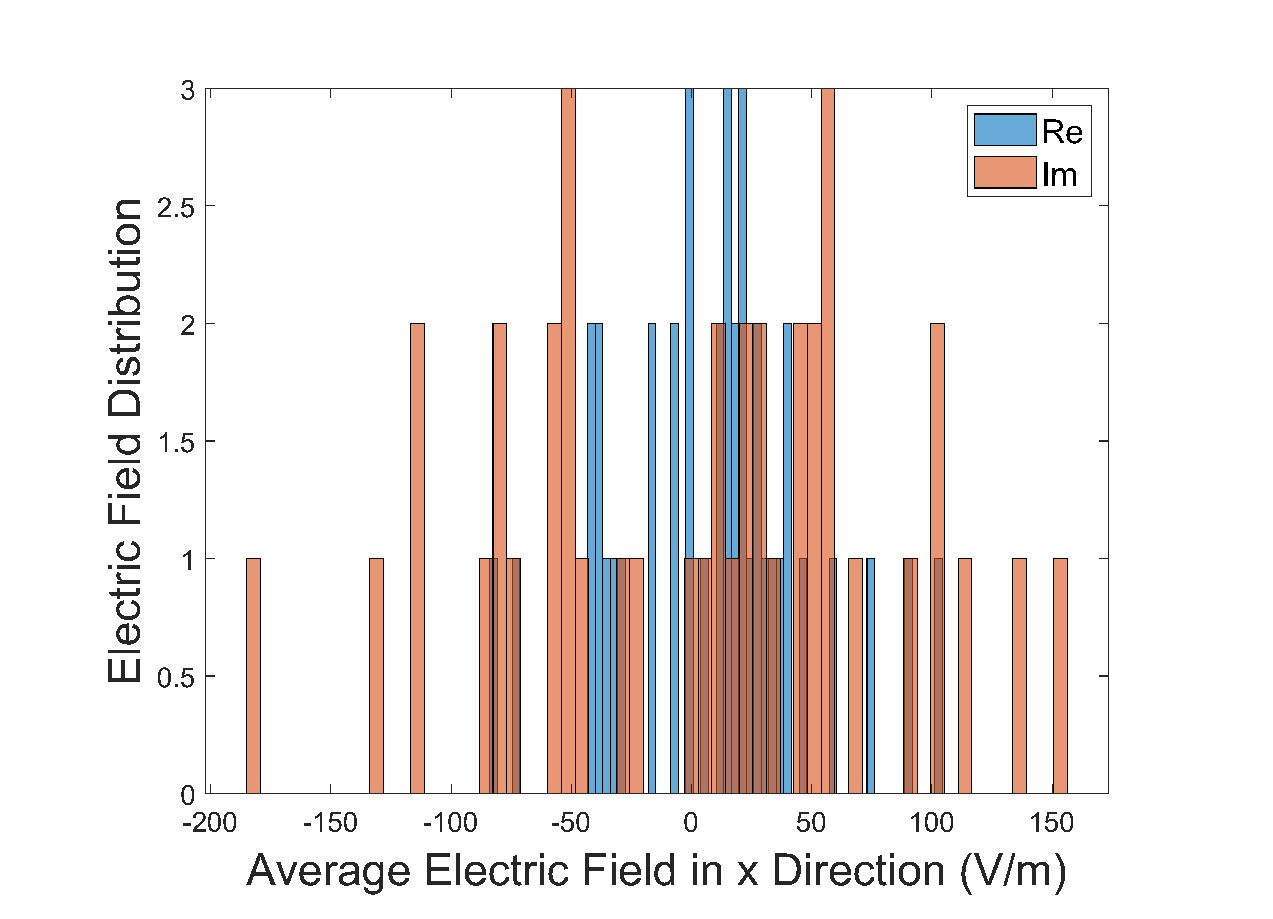
\includegraphics[bb=0bp 0bp 540bp 425bp,scale=0.28]{images/1StirrerOpt_xDir}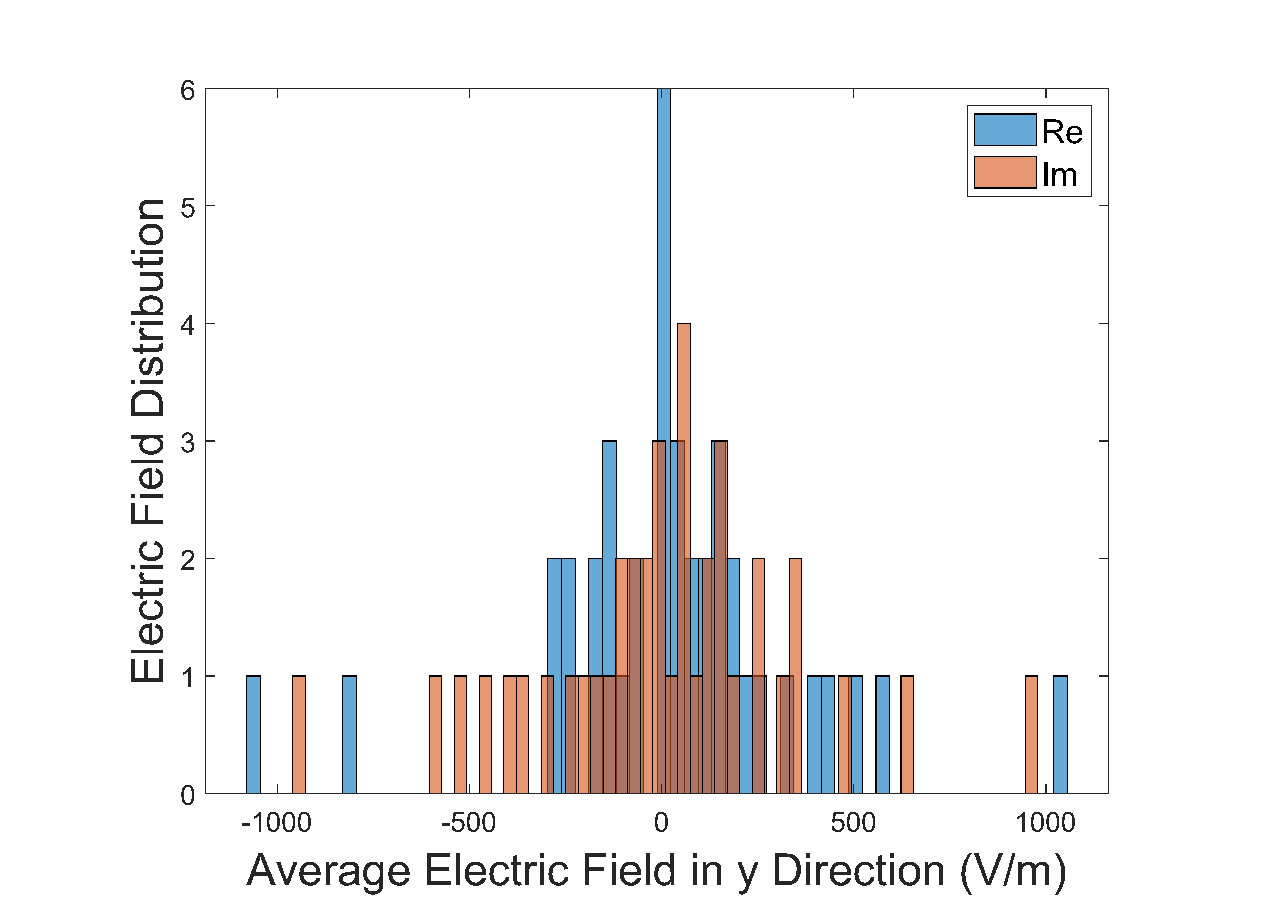
\includegraphics[bb=0bp 0bp 540bp 425bp,scale=0.28]{images/1StirrerOpt_yDir}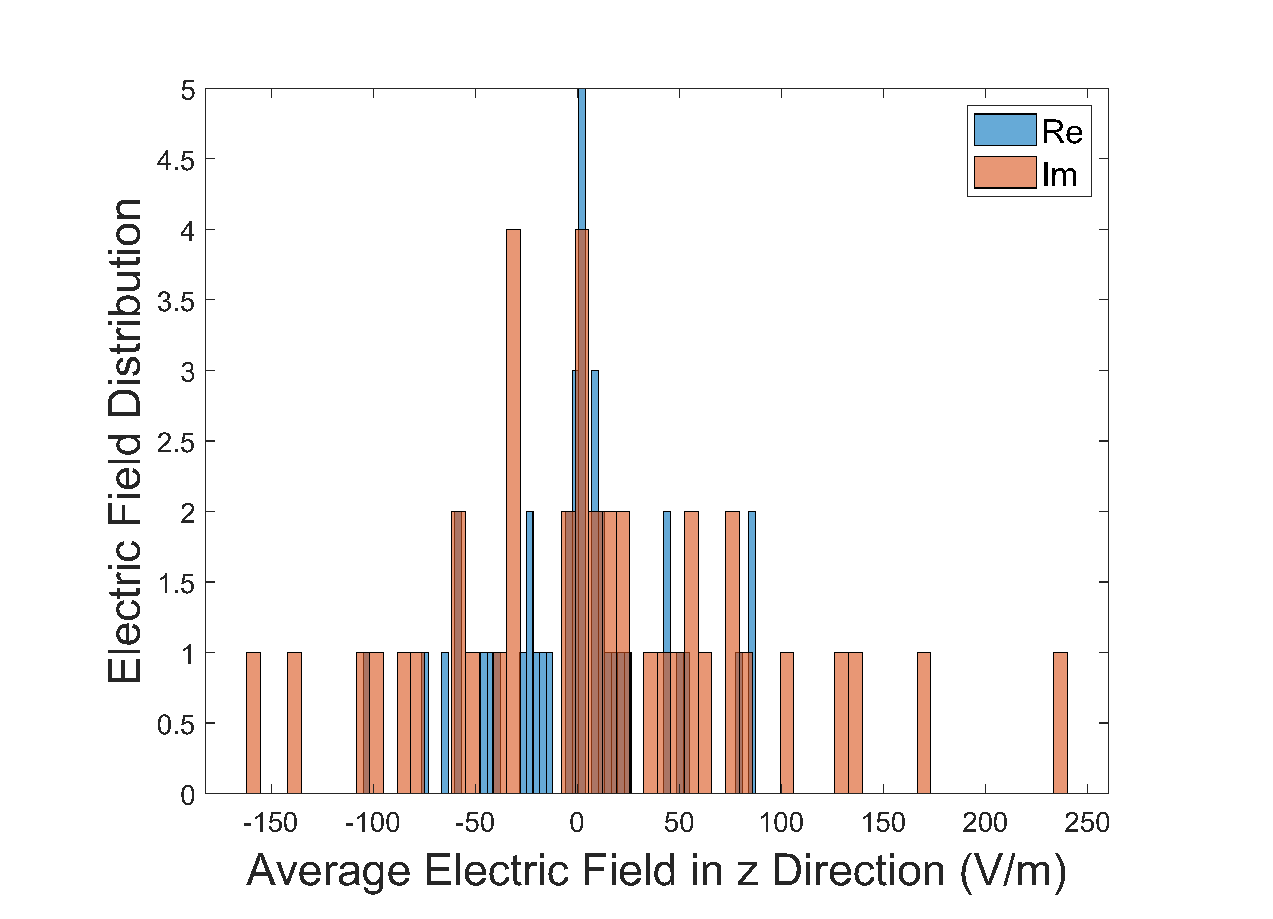
\includegraphics[bb=0bp 0bp 540bp 425bp,scale=0.28]{images/1StirrerOpt_zDir}
\par\end{centering}
\caption{\label{fig:simulation_OptSitrrer}Distribution of the average electric
field}
\end{figure}
The calculation produces the following values for the geometry optimized
parameters and $P$-values for the average electric field distribution.
\begin{table}[H]
\caption{\label{tab:P-value_OP}Resulting $P$-values of the simulation}

\centering{}%
\begin{tabular}{lccccccc}
 &  &  &  &  &  &  & \tabularnewline
\hline 
\hline 
Symbol &  & Optimized Values &  &  & Unit &  & Description\tabularnewline
\hline 
$tr_{1}y_{1}$ &  & $294$ &  &  & mm &  & distance\tabularnewline
$tr_{1}y_{2}$ &  & $28$ &  &  & mm &  & distance\tabularnewline
$tr_{2}y_{1}$ &  & $312$ &  &  & mm &  & distance\tabularnewline
$tr_{2}y_{2}$ &  & $19$ &  &  & mm &  & distance\tabularnewline
\hline 
\end{tabular} %
\begin{tabular}{lcccc}
 &  &  &  & \tabularnewline
\hline 
\hline 
Average Electric Field Distribution &  & Direction &  & $P$-value\tabularnewline
\hline 
\hline 
Real Part &  & $x$ &  & $0.4131$\tabularnewline
 &  & $y$ &  & $0.0019$\tabularnewline
 &  & $z$ &  & $0.3200$\tabularnewline
 &  &  &  & \tabularnewline
Imaginary Part &  & $x$ &  & $0.8599$\tabularnewline
 &  & $y$ &  & $0.1038$\tabularnewline
 &  & $z$ &  & $0.4860$\tabularnewline
\hline 
\end{tabular}
\end{table}
The $P$-values from the simulation with the optimized stirrer geometry
have improved when compared to the previous simulation but the desired
goal has not been reached for all $P$-values. Therefore, these results
lead to the introduction of two more optimized stirrers in remaining
x- and y-directions and the optimization of other relevant parameters.
\par\end{flushleft}

\begin{flushleft}
\begin{figure}[H]
\noindent \begin{centering}
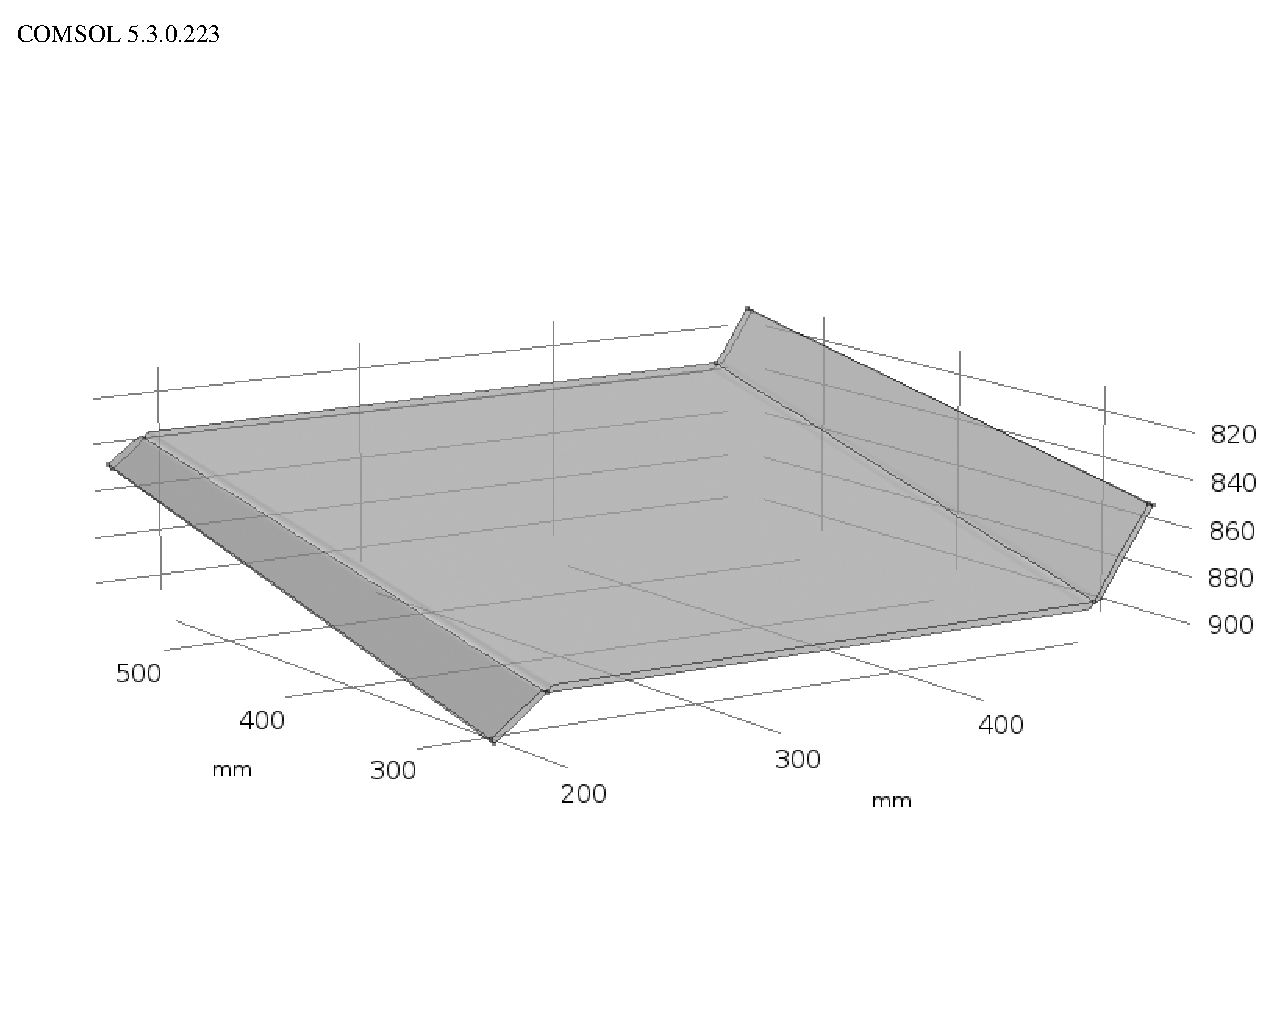
\includegraphics[bb=0bp 0bp 405bp 318.75bp,scale=0.4]{images/optstirrer}
\par\end{centering}
\caption{\label{fig:simulation_OptSitrrer1}The shape of the optimized stirrer}
\end{figure}
\par\end{flushleft}

The Fig. \ref{fig:simulation_OptSitrrer1} shows the resulting geometry
calculated by genetic algorithms.

\subsection{Result of the optimized shape for three stirrers}
\begin{flushleft}
In Fig.\ref{fig:MVK_dreiStr}, we observe the reverberation chamber
with three stirrer whose geometries have will later be optimized.
\begin{figure}[H]
\centering{}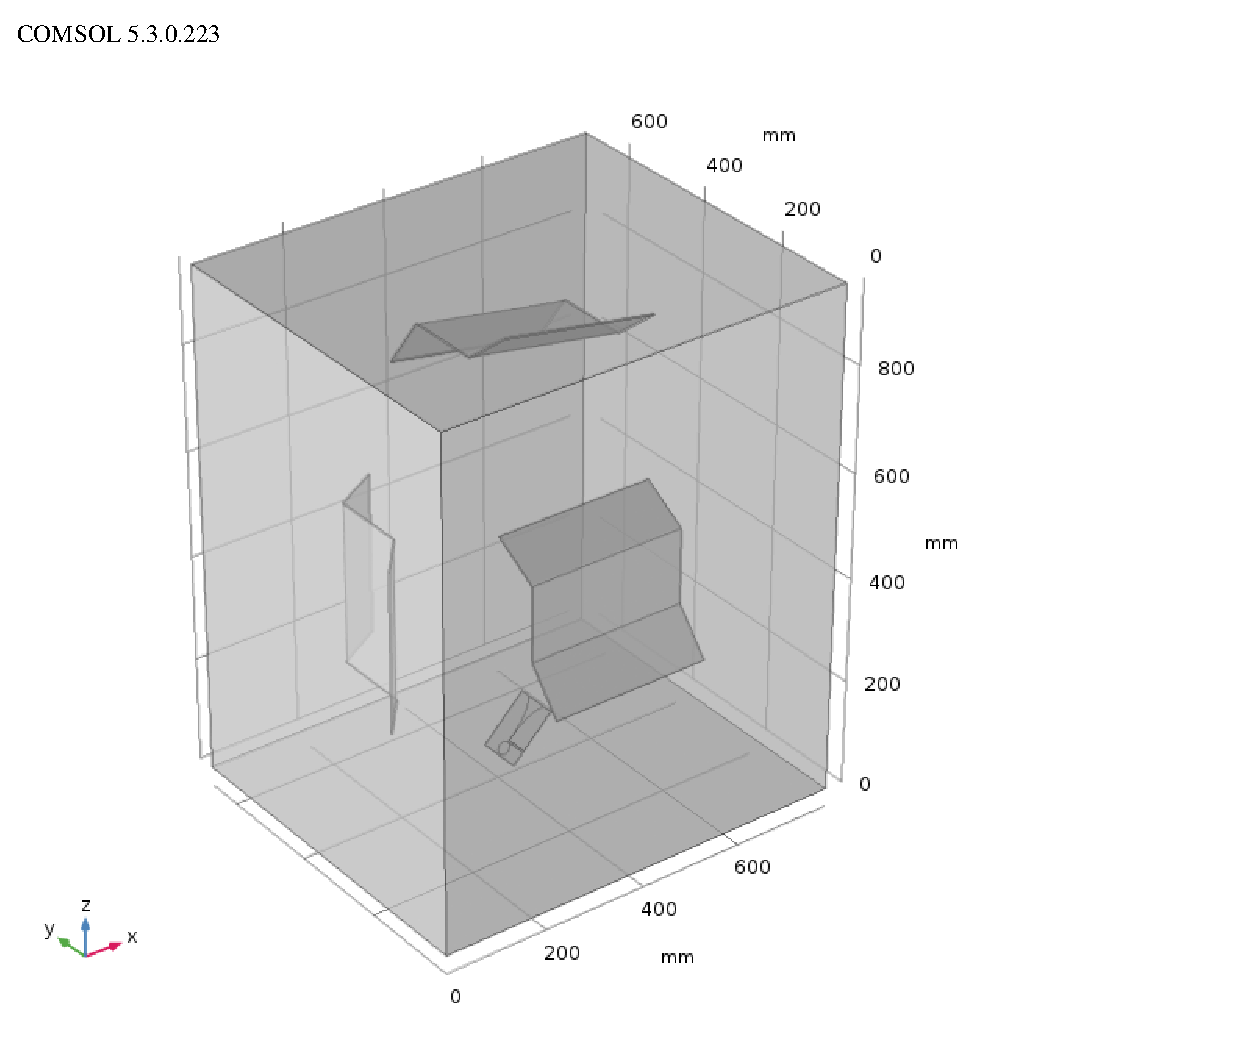
\includegraphics[bb=-67.5578bp 0bp 502.931bp 460bp,clip,scale=0.7]{images/3stirrers}\caption{\label{fig:MVK_dreiStr}Setup of the resonance chamber with three
stirrers, see Table \ref{tab:Model-parameters-3} for their postions}
\end{figure}
 The positions of all three stirrers are listed in Table \ref{tab:Model-parameters-3}.
\par\end{flushleft}

\begin{table}[H]
\centering{}\caption{Model parameters and values\label{tab:Model-parameters-3}}
\begin{tabular}{cllccccc}
 &  &  &  &  &  &  & \tabularnewline
\hline 
\hline 
Equipment & Parameter &  & Symbol &  & Value &  & Unit\tabularnewline
\hline 
Stirrer 1 & Position in x direction &  & $St_{x,1}$ &  & $0$ &  & mm\tabularnewline
 & Position in y direction &  & $St_{y,1}$ &  & $0$ &  & mm\tabularnewline
 & Position in z direction &  & $St_{z,1}$ &  & $860$ &  & mm\tabularnewline
Stirrer 2 & Position in x direction &  & $St_{x,2}$ &  & $0$ &  & mm\tabularnewline
 & Position in y direction &  & $St_{y,2}$ &  & $100$ &  & mm\tabularnewline
 & Position in z direction &  & $St_{z,2}$ &  & $0$ &  & mm\tabularnewline
Stirrer 3 & Position in x direction &  & $St_{x,3}$ &  & $100$ &  & mm\tabularnewline
 & Position in y direction &  & $St_{y,3}$ &  & $0$ &  & mm\tabularnewline
 & Position in z direction &  & $St_{z,3}$ &  & $0$ &  & mm\tabularnewline
\hline 
\end{tabular}
\end{table}
The parameters that have been chosen to be optimized are the shape
of the wings for all three stirrers inside the chamber. The newly
formulated fitness function for these selected parameters is

\begin{equation}
F_{P}=\sqrt{\overset{6}{\underset{i=1}{\sum}}\left|P_{i}\left(tr_{11}y_{1},...,tr_{23}y_{2}\right)-1\right|^{2}}\rightarrow\mathrm{min}.
\end{equation}
A new solution space for the three stirrers is specified in Table
\ref{tab:Solution-space-for-3}.
\begin{flushleft}
\begin{table}[H]
\caption{\label{tab:Solution-space-for-3}Solution space for genetic algorithms}

\centering{}%
\begin{tabular}{lllcccccccc}
 &  &  &  &  &  &  &  &  &  & \tabularnewline
\hline 
\hline 
Equipment &  & Symbol &  & Range &  & Step size &  & Unit &  & Description\tabularnewline
\hline 
Stirrer 1 &  & $tr_{11}y_{1}$ &  & $\left[\begin{array}{cc}
240 & 330\end{array}\right]$ &  & $9$ &  & mm &  & stirrer wing distance 1\tabularnewline
 &  & $tr_{11}y_{2}$ &  & $\left[\begin{array}{cc}
240 & 330\end{array}\right]$ &  & $9$ &  & mm &  & stirrer wing distance 2\tabularnewline
 &  & $tr_{21}y_{1}$ &  & $\left[\begin{array}{cc}
10 & 100\end{array}\right]$ &  & $9$ &  & mm &  & stirrer wing distance 3\tabularnewline
 &  & $tr_{21}y_{2}$ &  & $\left[\begin{array}{cc}
10 & 100\end{array}\right]$ &  & $9$ &  & mm &  & stirrer wing distance 4\tabularnewline
Stirrer 2 &  & $tr_{12}y_{1}$ &  & $\left[\begin{array}{cc}
240 & 330\end{array}\right]$ &  & $9$ &  & mm &  & stirrer wing distance 1\tabularnewline
 &  & $tr_{12}y_{2}$ &  & $\left[\begin{array}{cc}
240 & 330\end{array}\right]$ &  & $9$ &  & mm &  & stirrer wing distance 2\tabularnewline
 &  & $tr_{22}y_{1}$ &  & $\left[\begin{array}{cc}
10 & 100\end{array}\right]$ &  & $9$ &  & mm &  & stirrer wing distance 3\tabularnewline
 &  & $tr_{22}y_{2}$ &  & $\left[\begin{array}{cc}
10 & 100\end{array}\right]$ &  & $9$ &  & mm &  & stirrer wing distance 4\tabularnewline
Stirrer 3 &  & $tr_{13}y_{1}$ &  & $\left[\begin{array}{cc}
240 & 330\end{array}\right]$ &  & $9$ &  & mm &  & stirrer wing distance 1\tabularnewline
 &  & $tr_{13}y_{2}$ &  & $\left[\begin{array}{cc}
240 & 330\end{array}\right]$ &  & $9$ &  & mm &  & stirrer wing distance 2\tabularnewline
 &  & $tr_{23}y_{1}$ &  & $\left[\begin{array}{cc}
10 & 100\end{array}\right]$ &  & $9$ &  & mm &  & stirrer wing distance 3\tabularnewline
 &  & $tr_{23}y_{2}$ &  & $\left[\begin{array}{cc}
10 & 100\end{array}\right]$ &  & $9$ &  & mm &  & stirrer wing distance 4\tabularnewline
\hline 
\end{tabular}
\end{table}
As previously explained, a population with the chosen size of $18$
individuals and $7$ generations is generated through the algorithm.
Fig. \ref{fig:distr_gen-1} displays the value of the fitness function
for each generation. 
\begin{figure}[H]
\noindent \begin{centering}
\includegraphics[scale=0.4]{images/fitness3stirrers}
\par\end{centering}
\caption{\label{fig:distr_gen-1} Fitness value of the chosen population size
of $18$ individuals and $7$ generations}
\end{figure}
The simulation conditions, measurements taken for $40$ stirrer positions
and $9$ different points spaced out within the chamber, remain the
same. The histograms on Fig. \ref{fig:simulation_3Opt} present the
average electric field distribution in all directions for real and
imaginary parts.
\par\end{flushleft}

\begin{figure}[H]
\noindent \begin{centering}
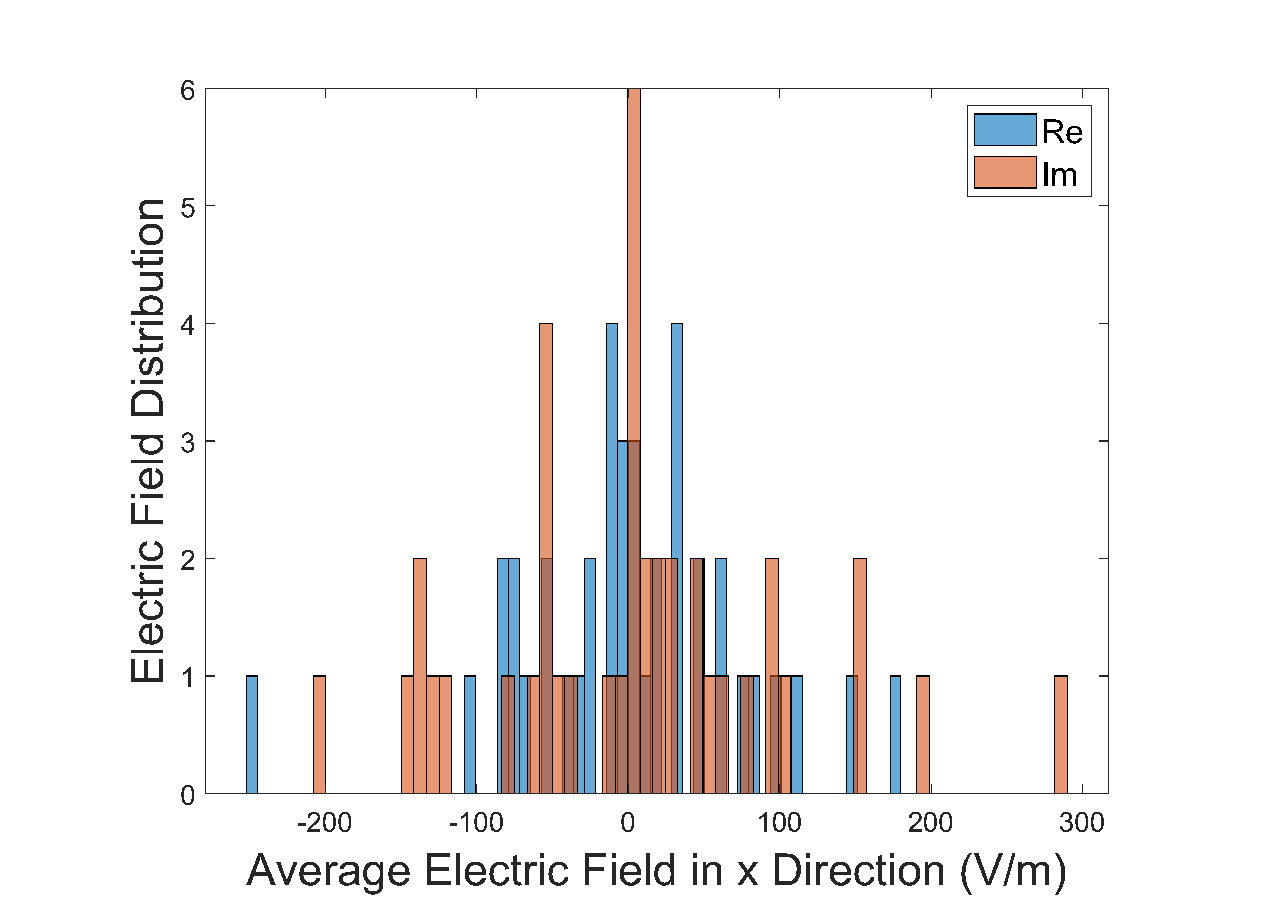
\includegraphics[bb=0bp 0bp 540bp 425bp,scale=0.28]{images/3StirrerOpt_xDir}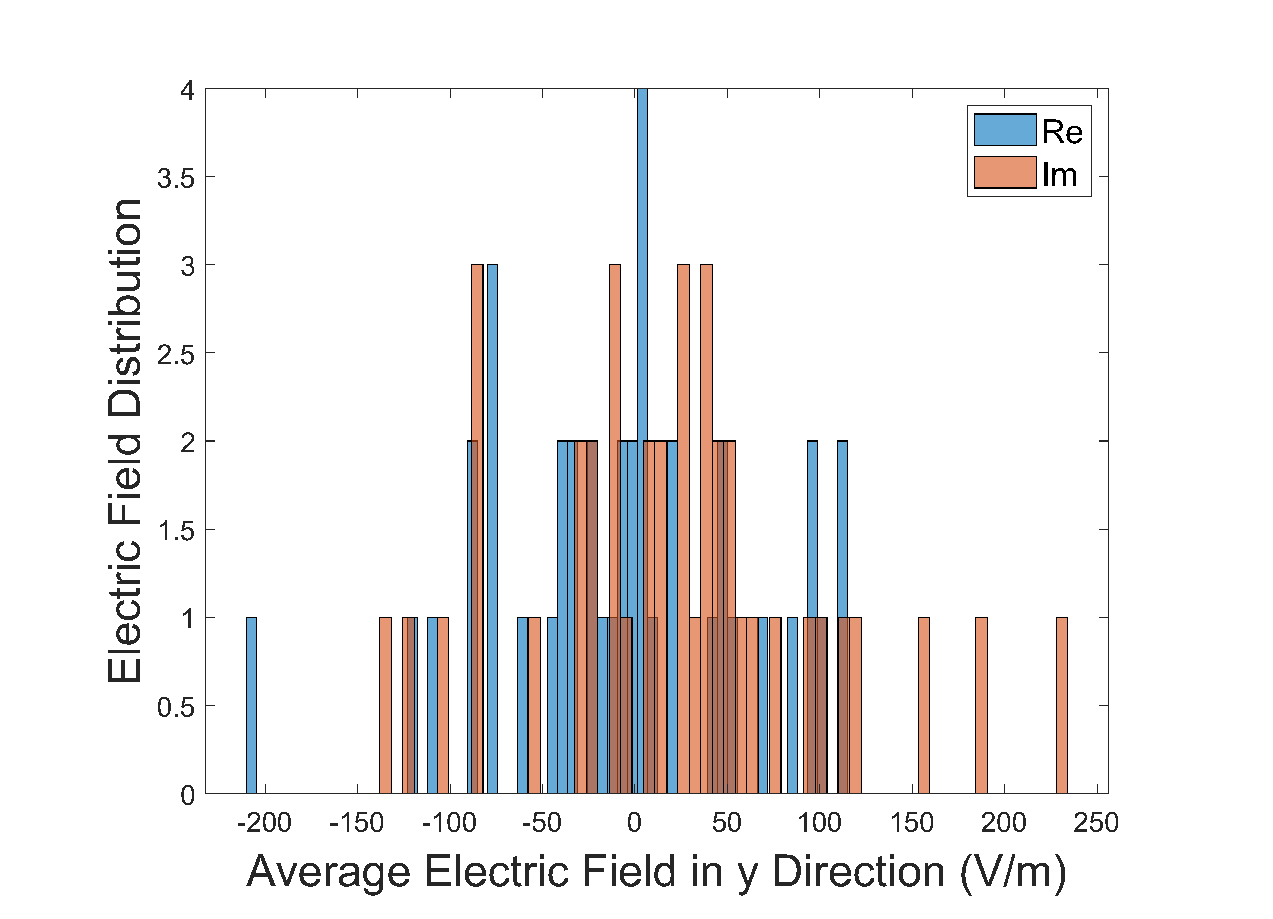
\includegraphics[bb=0bp 0bp 540bp 425bp,scale=0.28]{images/3StirrerOpt_yDir}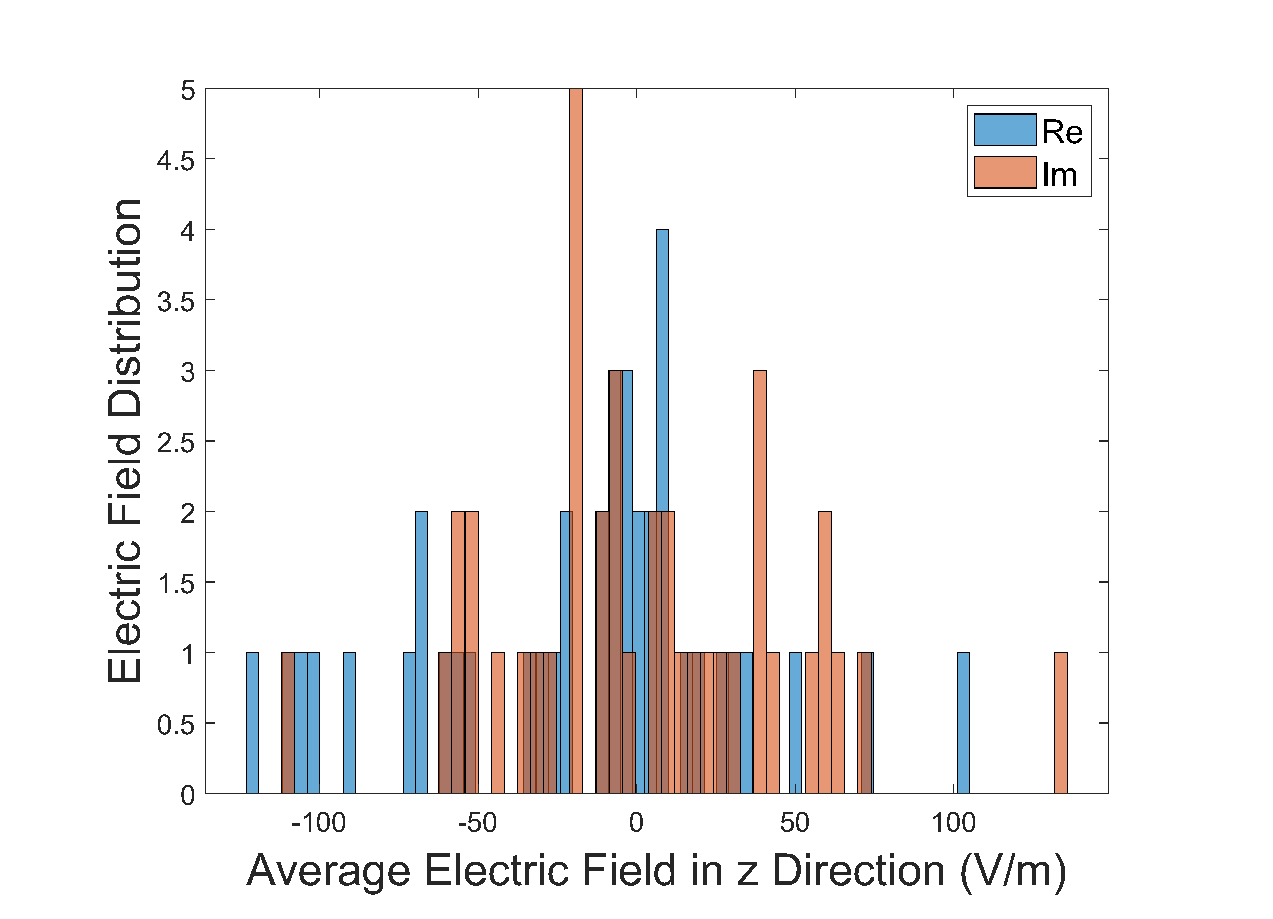
\includegraphics[bb=0bp 0bp 540bp 425bp,scale=0.28]{images/3StirrerOpt_zDir}
\par\end{centering}
\caption{\label{fig:simulation_3Opt}Distribution of the average electric field}
\end{figure}

\begin{table}[H]
\caption{\label{tab:P-value_3OPt}Resulting $P$-values of the simulation}

\centering{}%
\begin{tabular}{lccccc}
 &  &  &  &  & \tabularnewline
\hline 
\hline 
Symbol &  & Optimized Values &  &  & Unit\tabularnewline
\hline 
$tr_{11}y_{1}$ &  & $276$ &  &  & mm\tabularnewline
$tr_{11}y_{2}$ &  & $240$ &  &  & mm\tabularnewline
$tr_{21}y_{1}$ &  & $73$ &  &  & mm\tabularnewline
$tr_{21}y_{2}$ &  & $91$ &  &  & mm\tabularnewline
$tr_{12}y_{1}$ &  & $276$ &  &  & mm\tabularnewline
$tr_{12}y_{2}$ &  & $258$ &  &  & mm\tabularnewline
$tr_{22}y_{1}$ &  & $91$ &  &  & mm\tabularnewline
$tr_{22}y_{2}$ &  & $28$ &  &  & mm\tabularnewline
$tr_{13}y_{1}$ &  & $321$ &  &  & mm\tabularnewline
$tr_{13}y_{2}$ &  & $312$ &  &  & mm\tabularnewline
$tr_{23}y_{1}$ &  & $64$ &  &  & mm\tabularnewline
$tr_{23}y_{2}$ &  & $91$ &  &  & mm\tabularnewline
\hline 
\end{tabular} %
\begin{tabular}{lcccc}
 &  &  &  & \tabularnewline
\hline 
\hline 
Average Electric Field Distribution &  & Direction &  & $P$-value\tabularnewline
\hline 
\hline 
Real Part &  & $x$ &  & $0.0720$\tabularnewline
 &  & $y$ &  & $0.7291$\tabularnewline
 &  & $z$ &  & $0.0824$\tabularnewline
 &  &  &  & \tabularnewline
Imaginary Part &  & $x$ &  & $0.1880$\tabularnewline
 &  & $y$ &  & $0.4979$\tabularnewline
 &  & $z$ &  & $0.1378$\tabularnewline
\hline 
\end{tabular}
\end{table}

In conclusion, as seen in Table \ref{tab:P-value_3OPt}, all resulting
P-values have finally fulfilled the desired goal of at least 5\% in
all directions. This means that, when equiped with three optimised
stirrers, the ERC can achieve a normal distribution of the electric
field inside the chamber cavity with no further optimizations or changes
needed. Of note, is the observation that the optimized stirrers in
all cases have favored some symmetrical geometries than initially
predicted. This has additionally resulted in stirrers with flater
and wider reflective surfaces and smaller stirrer wings.

\subsection{Result for using different built-in objects in ERC}
\begin{flushleft}
Following several simulations and evaluations, the subsequent distributions
of the average electric field for both geometries were produced. Fig.
\ref{fig:simulation_kugel-1} represent the electric field distribution
for the model with half spheres in all three directions. 
\begin{figure}[H]
\noindent \begin{raggedright}
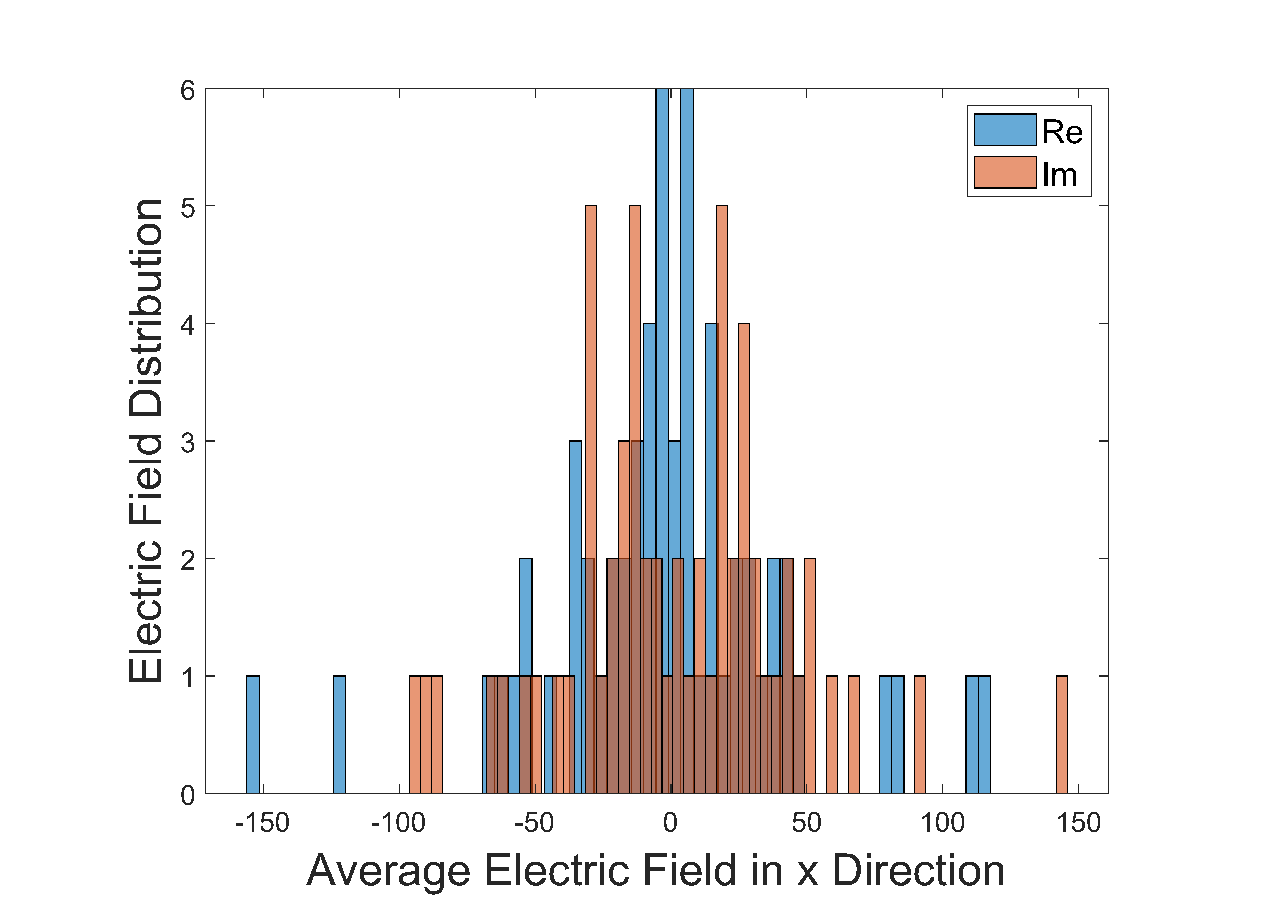
\includegraphics[bb=0bp 0bp 540bp 425bp,scale=0.28]{images/SphereXdirection}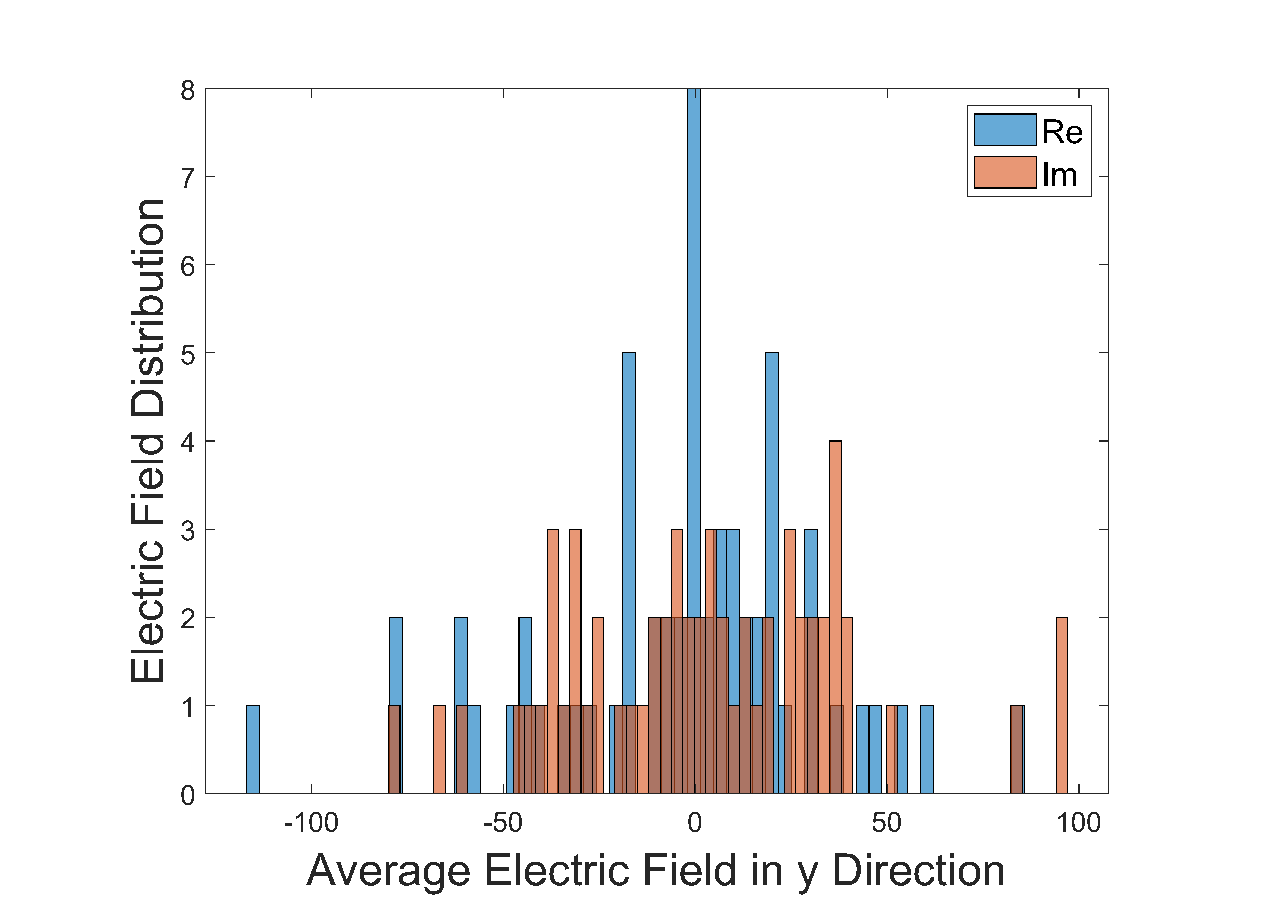
\includegraphics[bb=0bp 0bp 540bp 425bp,scale=0.28]{images/SphereYdirection}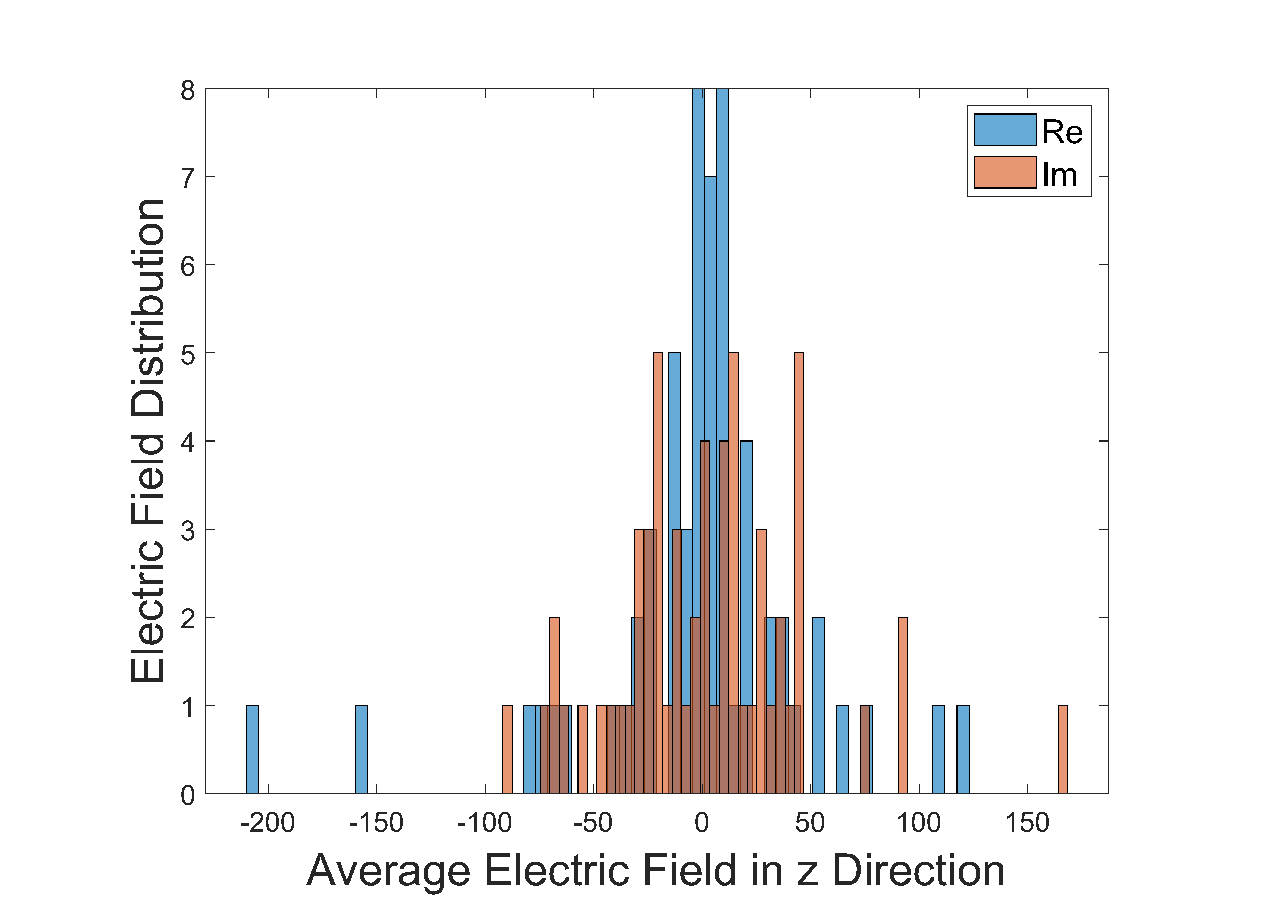
\includegraphics[bb=0bp 0bp 540bp 425bp,scale=0.28]{images/SphereZdirection}
\par\end{raggedright}
\caption{\label{fig:simulation_kugel-1}Distribution of the average electric
field for half spheres}
\end{figure}
Subsequently, the electric field distribution for the reverberation
chamber with the cones was simulated and represented in Fig. \ref{fig:simulation_kegel-1}.
This distribution is, as well, shown for all three directions and
for both real and imaginary part. All figures already serve to portray
the difference between the two models. At first sight, one can so
far determine that the distribution observed for figures relating
to the half spheres end up fulfilling expectations more so than those
of the cones. These observations are further proven true in Table
\ref{tab:P-value_both}. 
\begin{figure}[H]
\noindent \begin{raggedright}
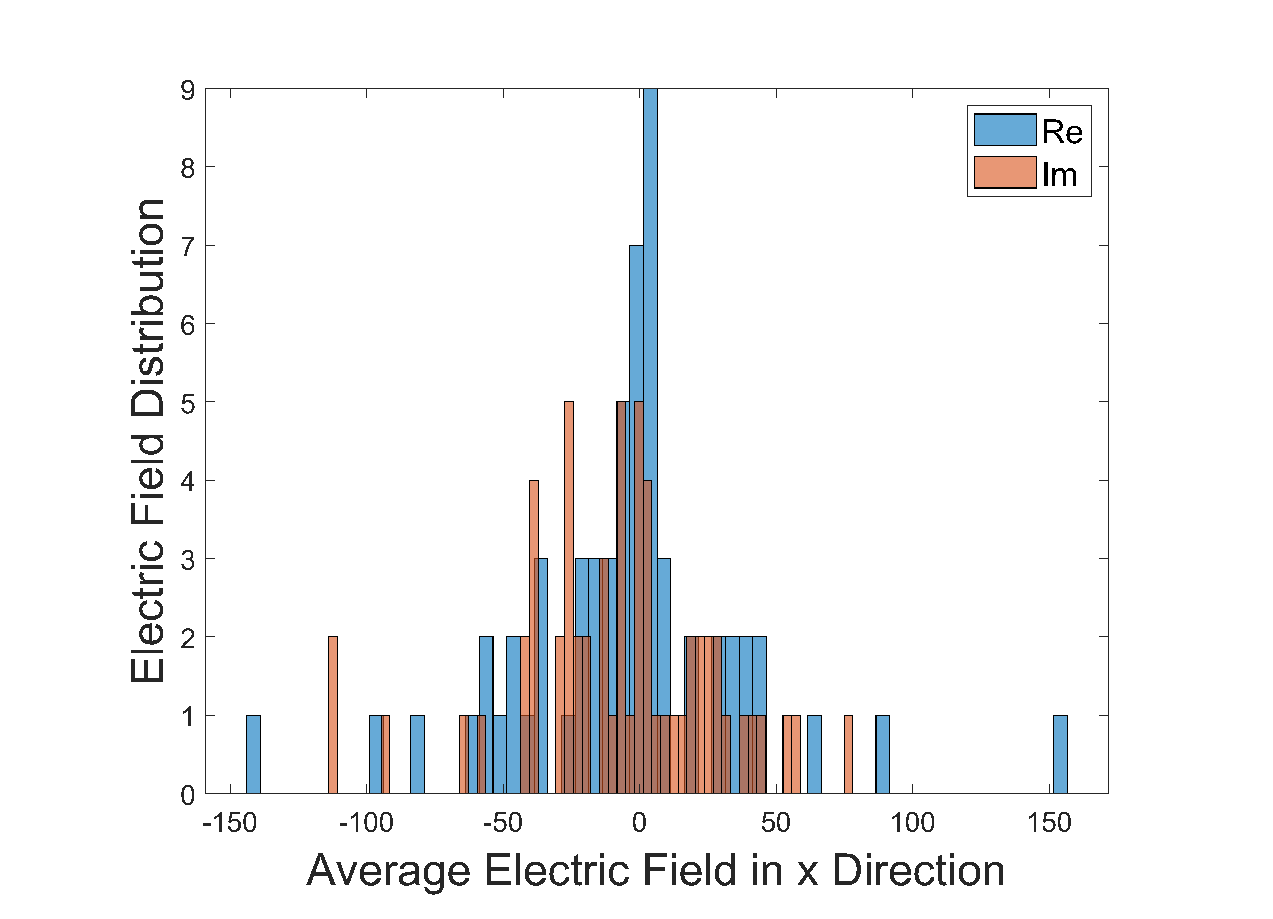
\includegraphics[bb=0bp 0bp 540bp 425bp,scale=0.28]{images/ConeXdirection}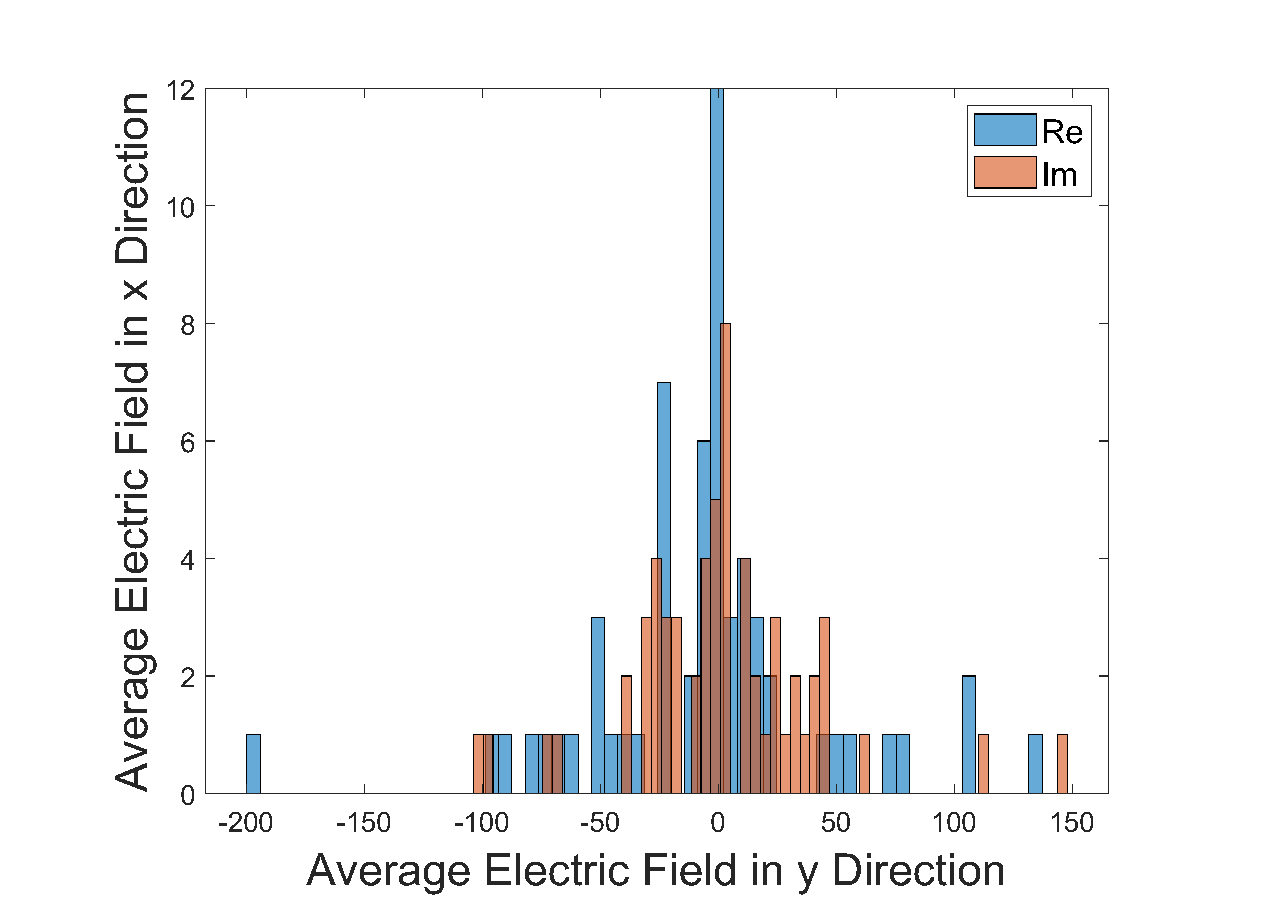
\includegraphics[bb=0bp 0bp 540bp 425bp,scale=0.28]{images/ConeYdirection}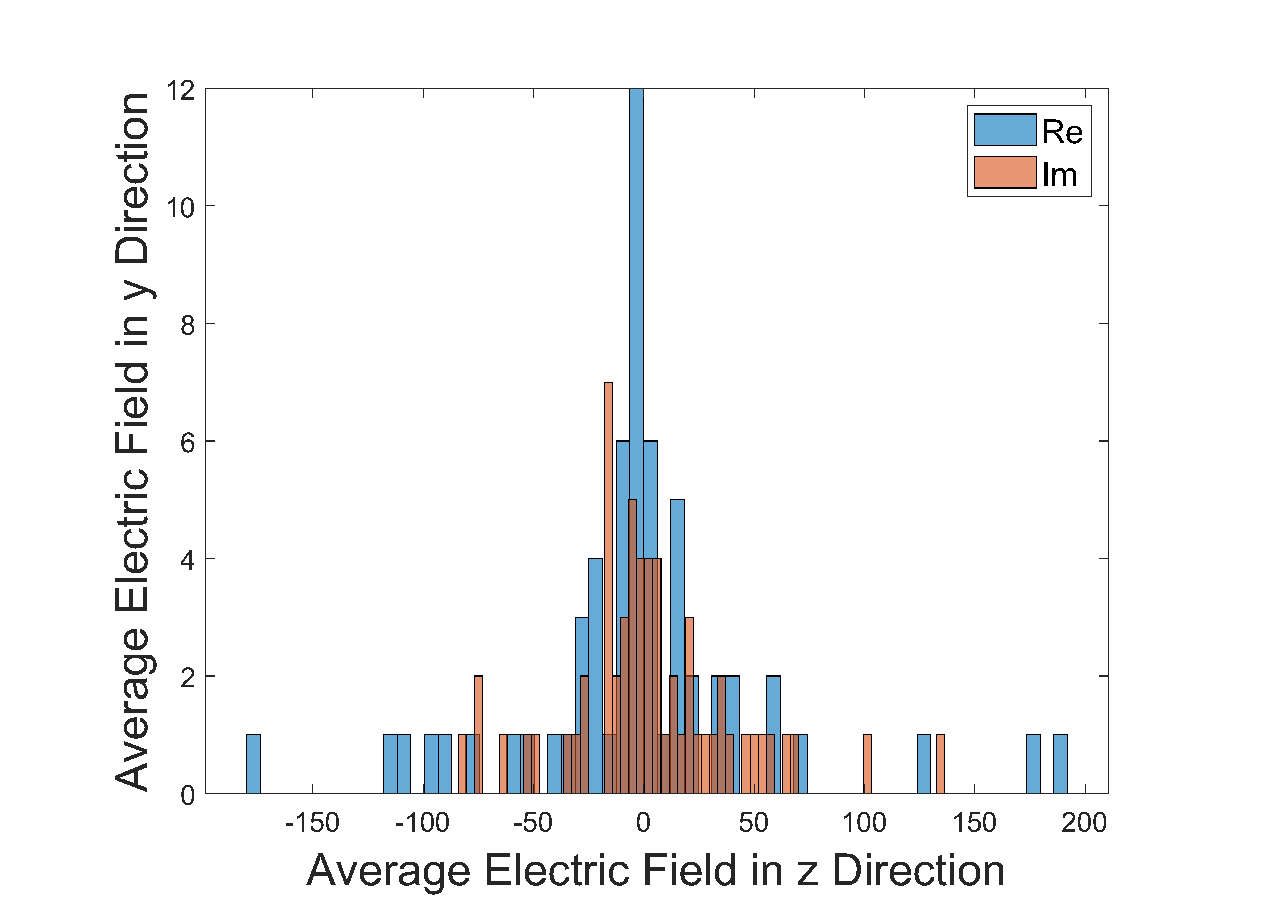
\includegraphics[bb=0bp 0bp 540bp 425bp,scale=0.28]{images/ConeZdirection}
\par\end{raggedright}
\caption{\label{fig:simulation_kegel-1}Distribution of the average electric
field for cones}
\end{figure}
The resulting P-values achieved by both models are listed below in
Table \ref{tab:P-value_both} and given for both real and imaginary
parts of the field.
\begin{table}[H]
\caption{\label{tab:P-value_both}Resulting P-values of the simulation}

\centering{}%
\begin{tabular}{lcccccc}
 &  &  &  &  &  & \tabularnewline
\hline 
\hline 
Average Electric Field Distribution &  & Direction &  & P-value of Half Sphere &  & P-value of Cone\tabularnewline
\hline 
\hline 
Real Part &  & $x$ &  & $0.0024$ &  & $3.4875\times10^{-4}$\tabularnewline
 &  & $y$ &  & $0.0513$ &  & $2.6074\times10^{-4}$\tabularnewline
 &  & $z$ &  & $6.2473\times10^{-6}$ &  & $2.7340\times10^{-5}$\tabularnewline
 &  &  &  &  &  & \tabularnewline
Imaginary Part &  & $x$ &  & $0.0893$ &  & $0.0294$\tabularnewline
 &  & $y$ &  & $0.2413$ &  & $9.0150\times10^{-4}$\tabularnewline
 &  & $z$ &  & $0.0095$ &  & $0.0085$\tabularnewline
\hline 
\end{tabular}
\end{table}
The P-values serve to emphasize the contrast of both geometries and,
thus, help in the choice of a better suited geometry for the ERC.
The P-values calculated for the half spheres are remarkably better
than those of the cones as half of them succeed the previously established
desired goal of at least $5$\%, whereas none of the values of the
cone simulation come even close to approaching the needed standard.
Nevertheless, the P-values are still not perfect and need to be optimized
further. 
\par\end{flushleft}

\section{Technical implementation}

The GA are implemented in Matlab and thus the initial population is
created. The values of the parameters are transmitted to Comsol via
Livelink, an interface between Matlab and Comsol. With these values,
Comsol simulates the model of the fuel cell and determines the cell
current for dierent voltages using finite element method. Matlab get
the data through Livelink and calculate the power curve. This is compared
with the indicated desired power curve and new values for the parameters
are calculated through GA. Finally, the parameters are transmitted
to Comsol again and the loop runs until the termination criteria are
reached.
\begin{flushleft}
The calculation time of the implementation is:
\par\end{flushleft}

\begin{equation}
T_{imp}=n_{I}*n_{G}*T_{sim}
\end{equation}
where $n_{P}$ is the number of individuals, $n_{G}$ the number of
generations and $T_{sim}$ the time for each simulation. In the mentioned
case, the size of the simulation included 8 individuals and 7 generations.
A computer with the power of 2.8 GHz CPU and 32 GB RAM was used. For
the simulation for fuel cell each simulation lasted in 1 minute and
45 seconds. The total calculation time yielded about 2 hours. The
opimization simulation of the optimized stirrer geometry and the performance
to optimized the shape of three stirrer yielded about $70$ hours.
The size of the simulation included $18$ individuals and $7$ generations.
\end{document}
